% !TEX TS-program = pdflatex
% !TEX encoding = UTF-8 Unicode

% This is a simple template for a LaTeX document using the "article" class.
% See "book", "report", "letter" for other types of document.

\documentclass[11pt]{article} % use larger type; default would be 10pt

\usepackage[utf8]{inputenc} % set input encoding (not needed with XeLaTeX)

%%% Examples of Article customizations
% These packages are optional, depending whether you want the features they provide.
% See the LaTeX Companion or other references for full information.

%%% PAGE DIMENSIONS
\usepackage{geometry} % to change the page dimensions
\geometry{a4paper} % or letterpaper (US) or a5paper or....
% \geometry{margin=2in} % for example, change the margins to 2 inches all round
% \geometry{landscape} % set up the page for landscape
%   read geometry.pdf for detailed page layout information

\usepackage{graphicx} % support the \includegraphics command and options
\usepackage{subcaption} % para subfiguras
\usepackage{caption}
\usepackage{float}

% \usepackage[parfill]{parskip} % Activate to begin paragraphs with an empty line rather than an indent

%%% PACKAGES
\usepackage{booktabs} % for much better looking tables
\usepackage{array} % for better arrays (eg matrices) in maths
\usepackage{paralist} % very flexible & customisable lists (eg. enumerate/itemize, etc.)
\usepackage{verbatim} % adds environment for commenting out blocks of text & for better verbatim
% \usepackage{subfig} % make it possible to include more than one captioned figure/table in a single float
% These packages are all incorporated in the memoir class to one degree or another...
\usepackage{amsmath,amssymb}

%%% HEADERS & FOOTERS
\usepackage{fancyhdr} % This should be set AFTER setting up the page geometry
\pagestyle{fancy} % options: empty , plain , fancy
\renewcommand{\headrulewidth}{0pt} % customise the layout...
\lhead{}\chead{}\rhead{}
\lfoot{}\cfoot{\thepage}\rfoot{}

%%% SECTION TITLE APPEARANCE
\usepackage{sectsty}
\allsectionsfont{\sffamily\mdseries\upshape} % (See the fntguide.pdf for font help)
% (This matches ConTeXt defaults)

%%% ToC (table of contents) APPEARANCE
\usepackage[nottoc,notlof,notlot]{tocbibind} % Put the bibliography in the ToC
\usepackage[titles,subfigure]{tocloft} % Alter the style of the Table of Contents
\renewcommand{\cftsecfont}{\rmfamily\mdseries\upshape}
\renewcommand{\cftsecpagefont}{\rmfamily\mdseries\upshape} % No bold!

\usepackage{hyperref}
\usepackage{cleveref}
%%% END Article customizations

%%% The "real" document content comes below...
\begin{document}

\title{Trabajo Fin de Máster}
\author{Jorge Zorrilla Prieto}

%\date{} % Activate to display a given date or no date (if empty),
         % otherwise the current date is printed 


\maketitle

% \begin{titlepage}
%     \centering
%     {\scshape\LARGE Universidad Carlos III de Madrid \par}
%     \vspace{2cm}
%     {\huge\bfseries Trabajo Fin de Máster \par}
%     \vspace{1.5cm}
%     {\Large\itshape Jorge Zorrilla Prieto \par}
%     \begin{figure}[h] % [h] = here, [t] = top, [b] = bottom
%         \centering
%         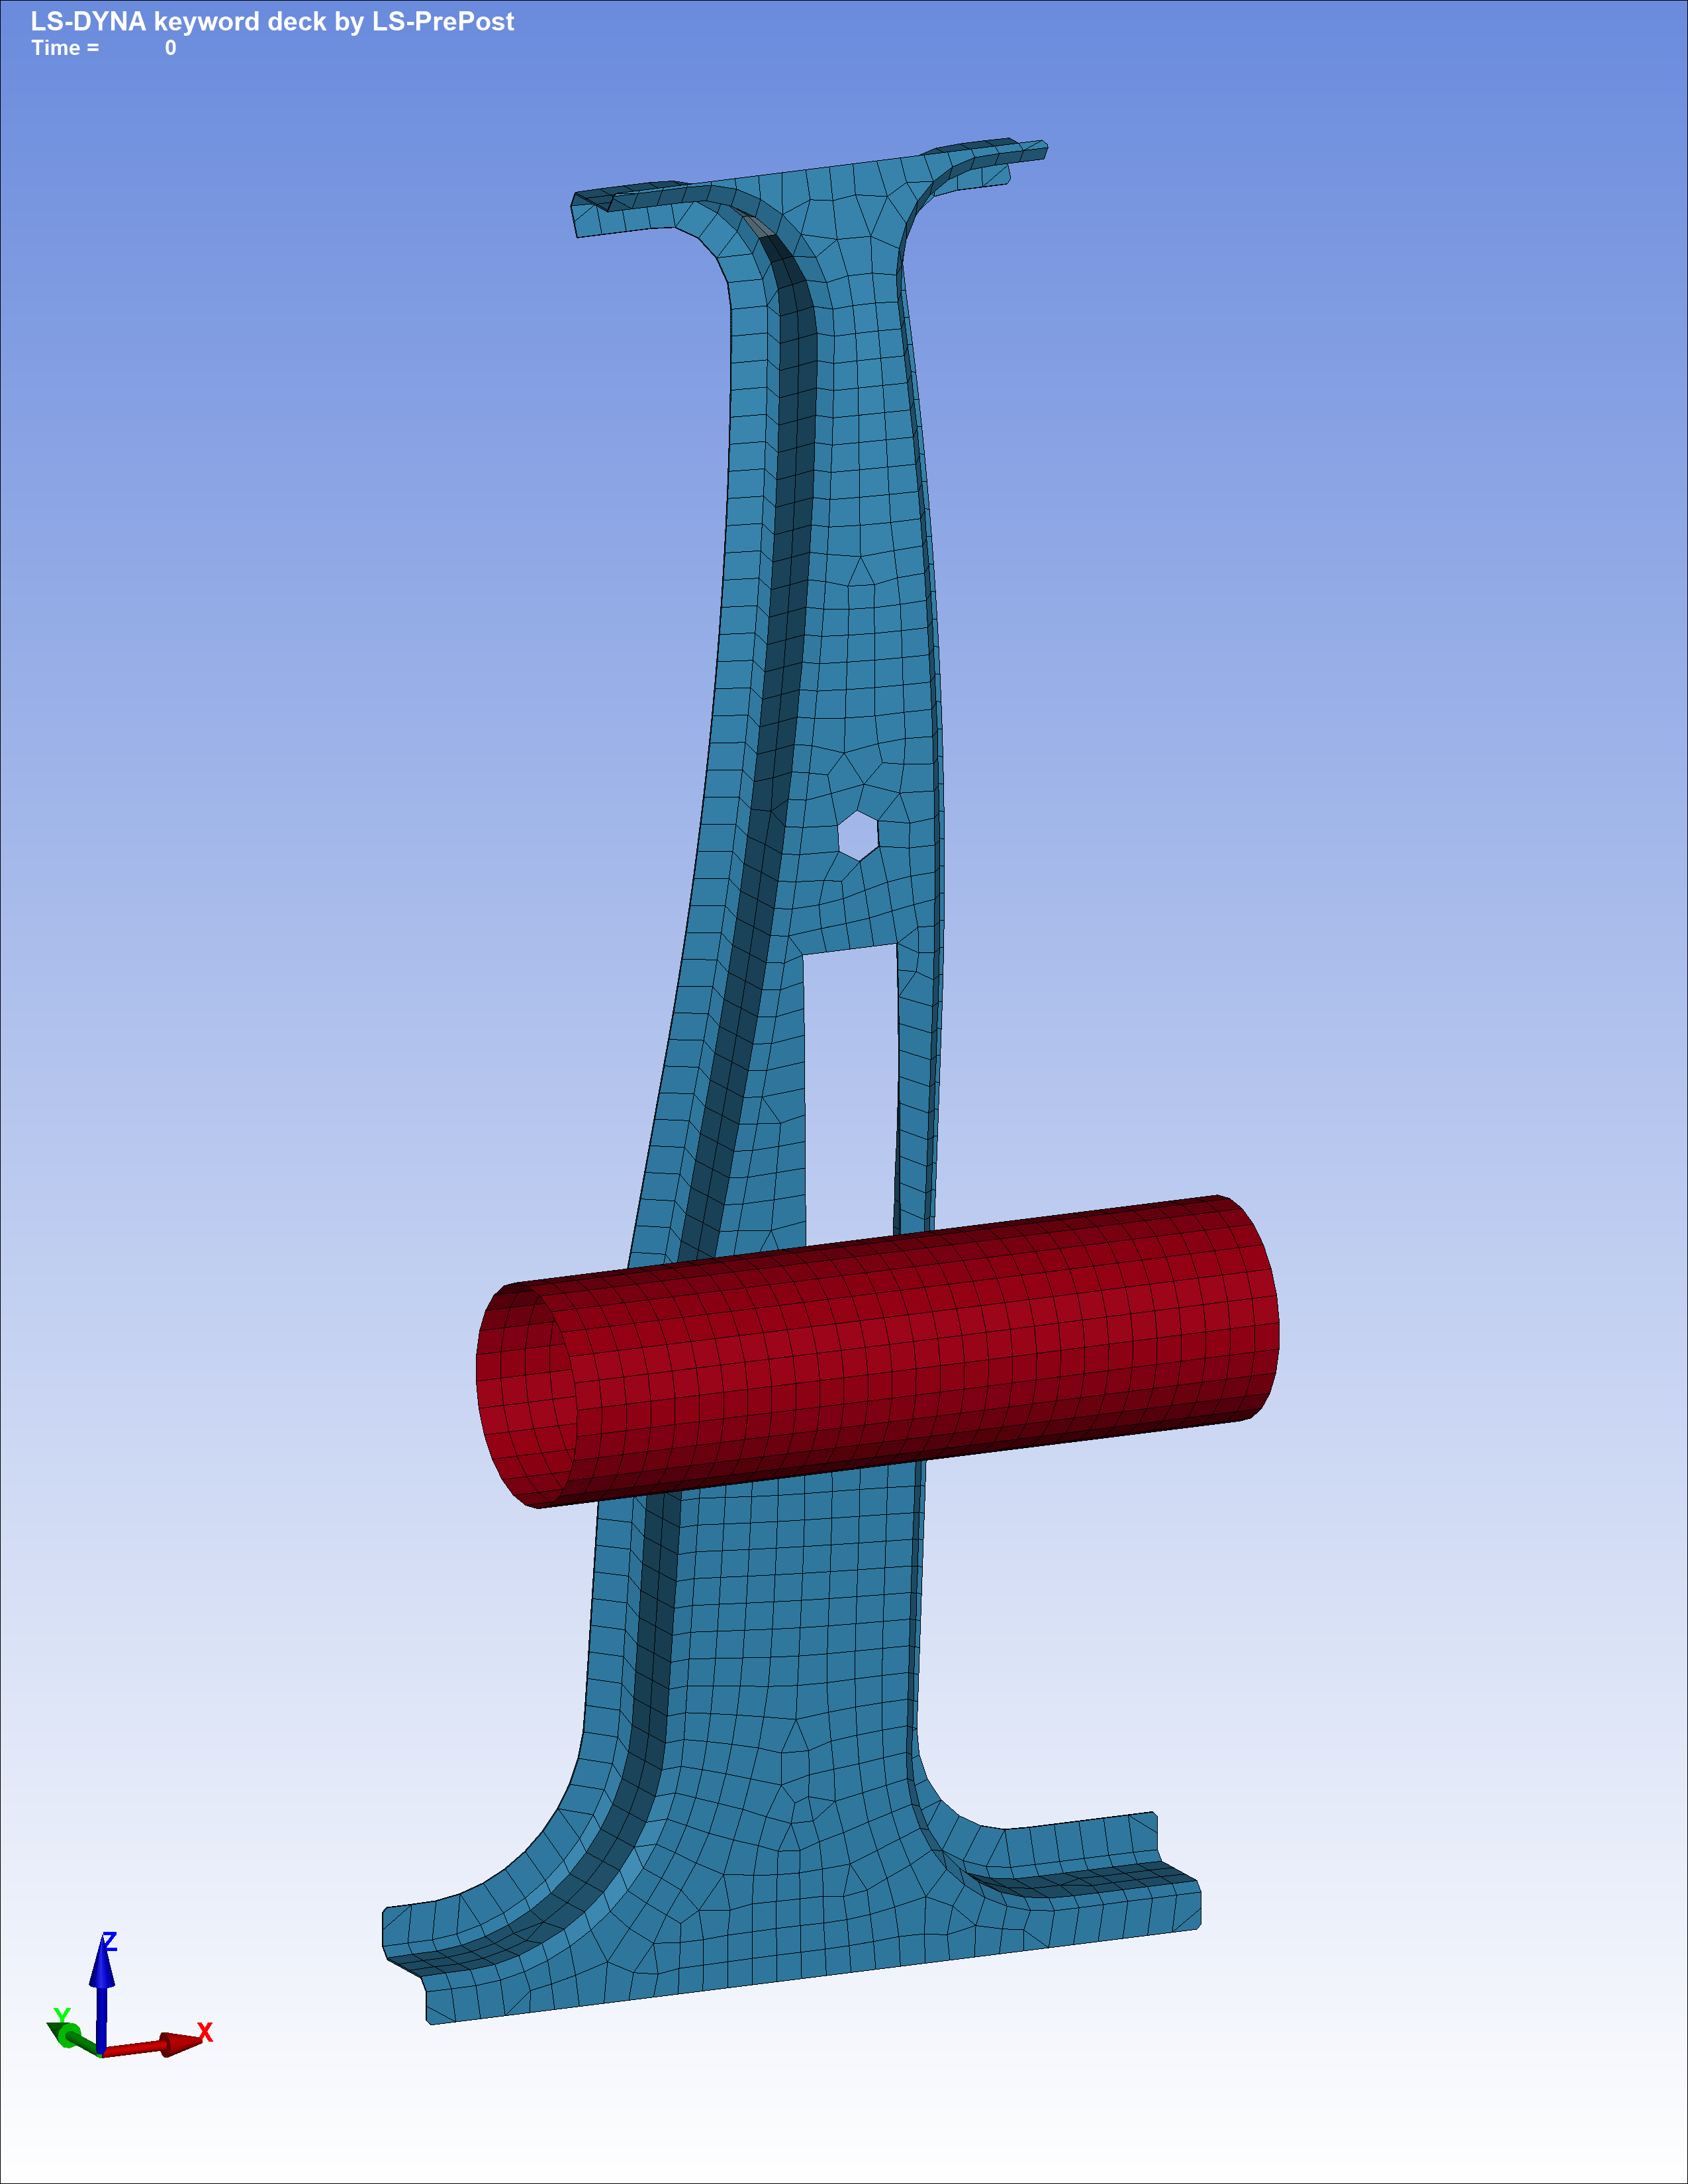
\includegraphics[scale=0.15]{images/modelo-inicial.png} 
%     \end{figure}

%     \vfill
%     Tuto: Rafael Vázquez Hernández \par
%     \vspace{0.8cm}
%     {\large Septiembre 2025 \par}
% \end{titlepage}

\section{Introducción}
TBD

\section{Generación de las simulaciones de entrada}
Inicialmente planteamos como problema objetivo para la simulación el siguiente:
\newline
\newline
\textit{Simulación de impacto entre una estructura cilíndrica rígida de tipo shell con una velocidad inicial que impacta con un sólido tipo B-Pillar elásto-plástico también de tipo shell y que
se encuentra estático.}
\newline
\newline

A partir de este enunciado desarrollaremos durante esta sección la elección de los diferentes parámetros que usaremos para las simulaciones que servirán más adelante como \textit{input} al
modelo de GNNs.

\subsection{Elección de software}
De cara a realizar las simulaciones que se necesitarán más adelante para alimentar el modelo de IA, varias opciones estaban disponibles en el mercado. Inicialmente se plantearon 
por parte de la compañía las herramientas \textit{Abaqus}\cite{abaqus} de \textit{Dassault Systemes}, \textit{Pam-Crash}\cite{pam-crash} de \textit{ESI-Group}, \textit{LS-DYNA}\cite{ls-dyna-web} de la empresa \textit{ANSYS} y \textit{Nastran}
de \textit{Autodesk}\cite{nastran}. Debido a restricciones económicas para solicitar las licencias comerciales de estas compañias, se hace un estudio de sus licencias estudiantiles, si existieran. El resultado del 
estudio da como solución final \textit{LS-DYNA} debido a que era una de las pocas soluciones gratuitas ofrecidas por estás compañías y además la única donde las restricciones en cuanto al
tamaño máximo de las simulaciones (en cuanto a número de nodos) sobrepasaban nuestran necesidades.

\subsection{Sistema de Unidades}

A pesar de ser el Sistema Internacional (SI) en aplicaciones de ingeniería, en algunos software de simulación como \textit{ABAQUS} o \textit{LS-DYNA} se usa el sistema basado en milímetros (\cref{tab:sistema-unidades}). 
Es por esto que escogemos este sistema a fin de evitar potenciales problemas de conversión de etapas posteriores del proyecto.

\begin{table}[h]
  \centering
  \begin{tabular}{l c}
    \toprule
    Magnitud & Unidad usada en el modelo \\
    \midrule
    Longitud & milímetro (mm) \\
    Masa & tonelada (tonne = $1000$ kg) \\
    Fuerza & Newton (N) \\
    Tiempo & segundo (s) \\
    Tensión / Módulo & megapascal (MPa = N/mm$^2$) \\
    Densidad & tonne/mm$^3$ \\
    \bottomrule
  \end{tabular}
  \caption{Sistema de unidades utilizado en las simulaciones.}
  \label{tab:sistema-unidades}
\end{table}


\subsection{Geometría}
Debido a la alta exigencia computacional que tienen los modelos de GNNs y en haras de obtener los mejores resultados posibles, limitamos nuestro planteamiento geométrico a uno lo más sencillo
posible pero técnicamente interesamente. Como sólido impactador tendremos un cilindro rígido (\cref{fig:cilindro}) y como B-Pillar partimos de un modelo de CAD sencillo que refleje con más o menos fidelidad a uno
de verdad (\cref{fig:b-pillar}). Además, a partir de la geometría base del B-Pillar, realizamos 100 geometrías adicionales en las que introducimos modificaciones en cuanto a tamaño, forma y número de agujeros.

\begin{figure}[H]
    \centering
    
    % --- fila 1 ---
    \begin{subfigure}{0.45\textwidth}
        \centering
        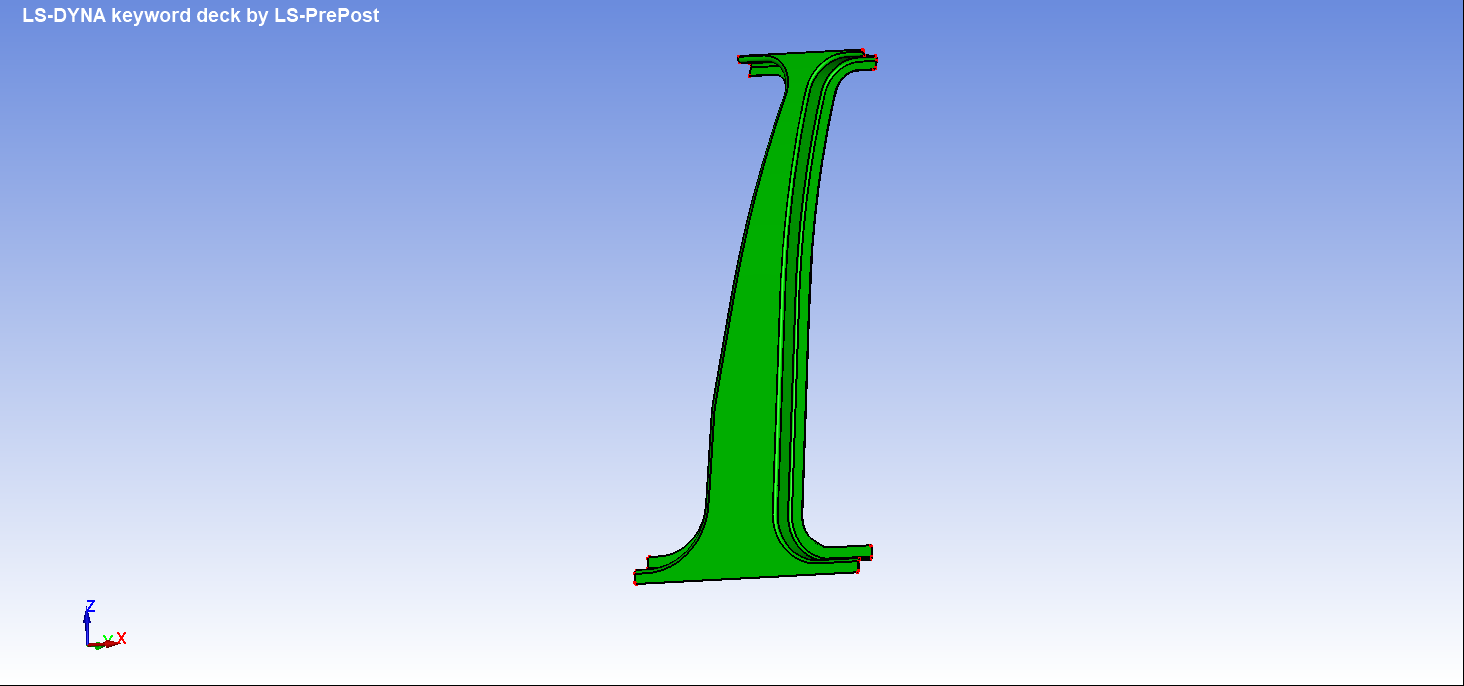
\includegraphics[width=\linewidth]{images/b-pillar.png}
        \caption{B-Pillar}\label{fig:b-pillar}
    \end{subfigure}
    \hfill
    \begin{subfigure}{0.45\textwidth}
        \centering
        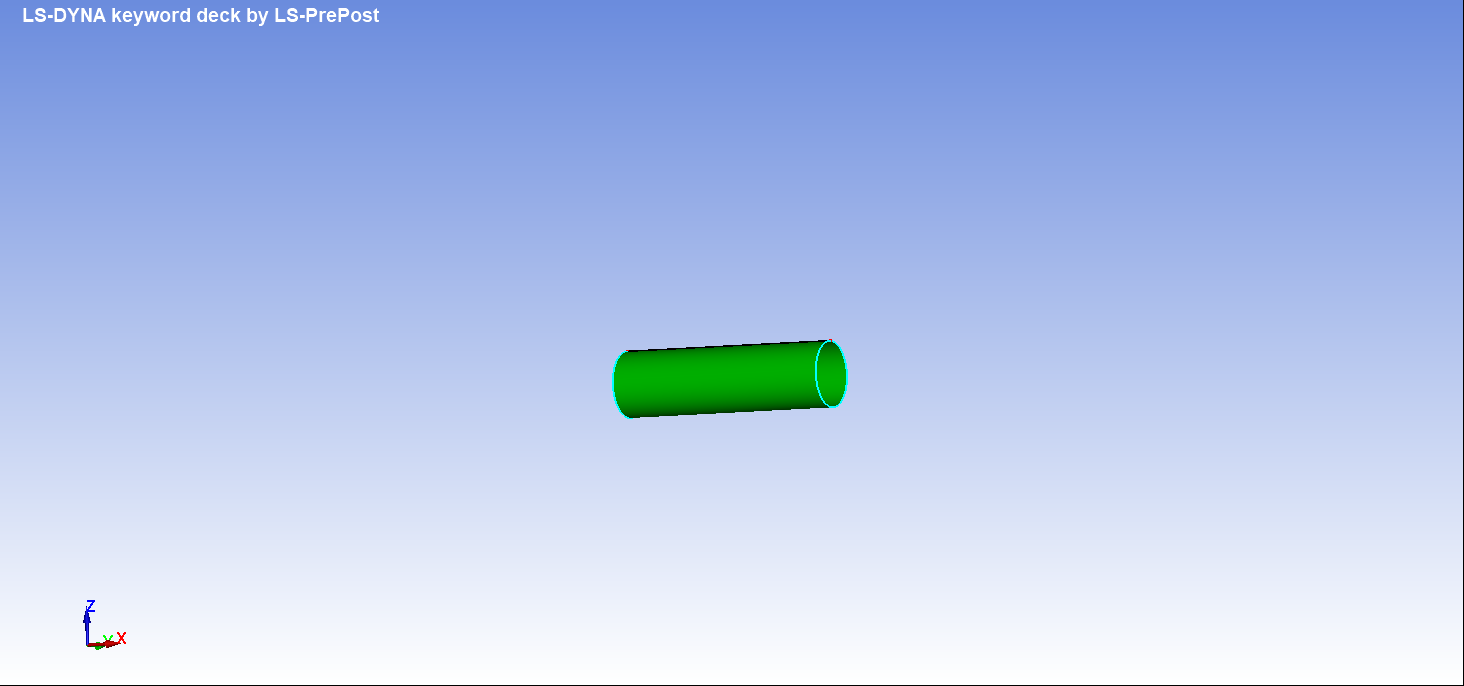
\includegraphics[width=\linewidth]{images/cilindro.png}
        \caption{Cilindro}\label{fig:cilindro}
        \end{subfigure}
    \caption{Geometrías iniciales.}\label{fig:geometria-inicial}
\end{figure}

\subsection{Mallado}
Definimos las dos geometrías anteriormente mencionadas como sólidos tipo \textit{shell} con el objetivo de tener unos modelos simplificados del problema sin un exceso de elementos en el problema
a tratar. Debido a la limitación de hardware mencionada anteriormente, limitamos la resolución de nuestro modelo a unos 5000 nodos por simulación. Tras haber realizado pruebas con diferentes resoluciones,
consideramos que una de unos 20 mm para elementos de tipo tanto triangular como tetrahédrico sirve como solución de compromiso con la que se puede capturar con fidelidad el especio alrededor de los agujeros 
creados (mayor requisito técnico) (\cref{fig:modelo-inicial}). Aplicamos este mallado por igual a los 100 modelos con las 100 variaciones del B-Pillar (\cref{fig:variaciones-geometry}).

\begin{figure}[H] % [h] = here, [t] = top, [b] = bottom
\centering
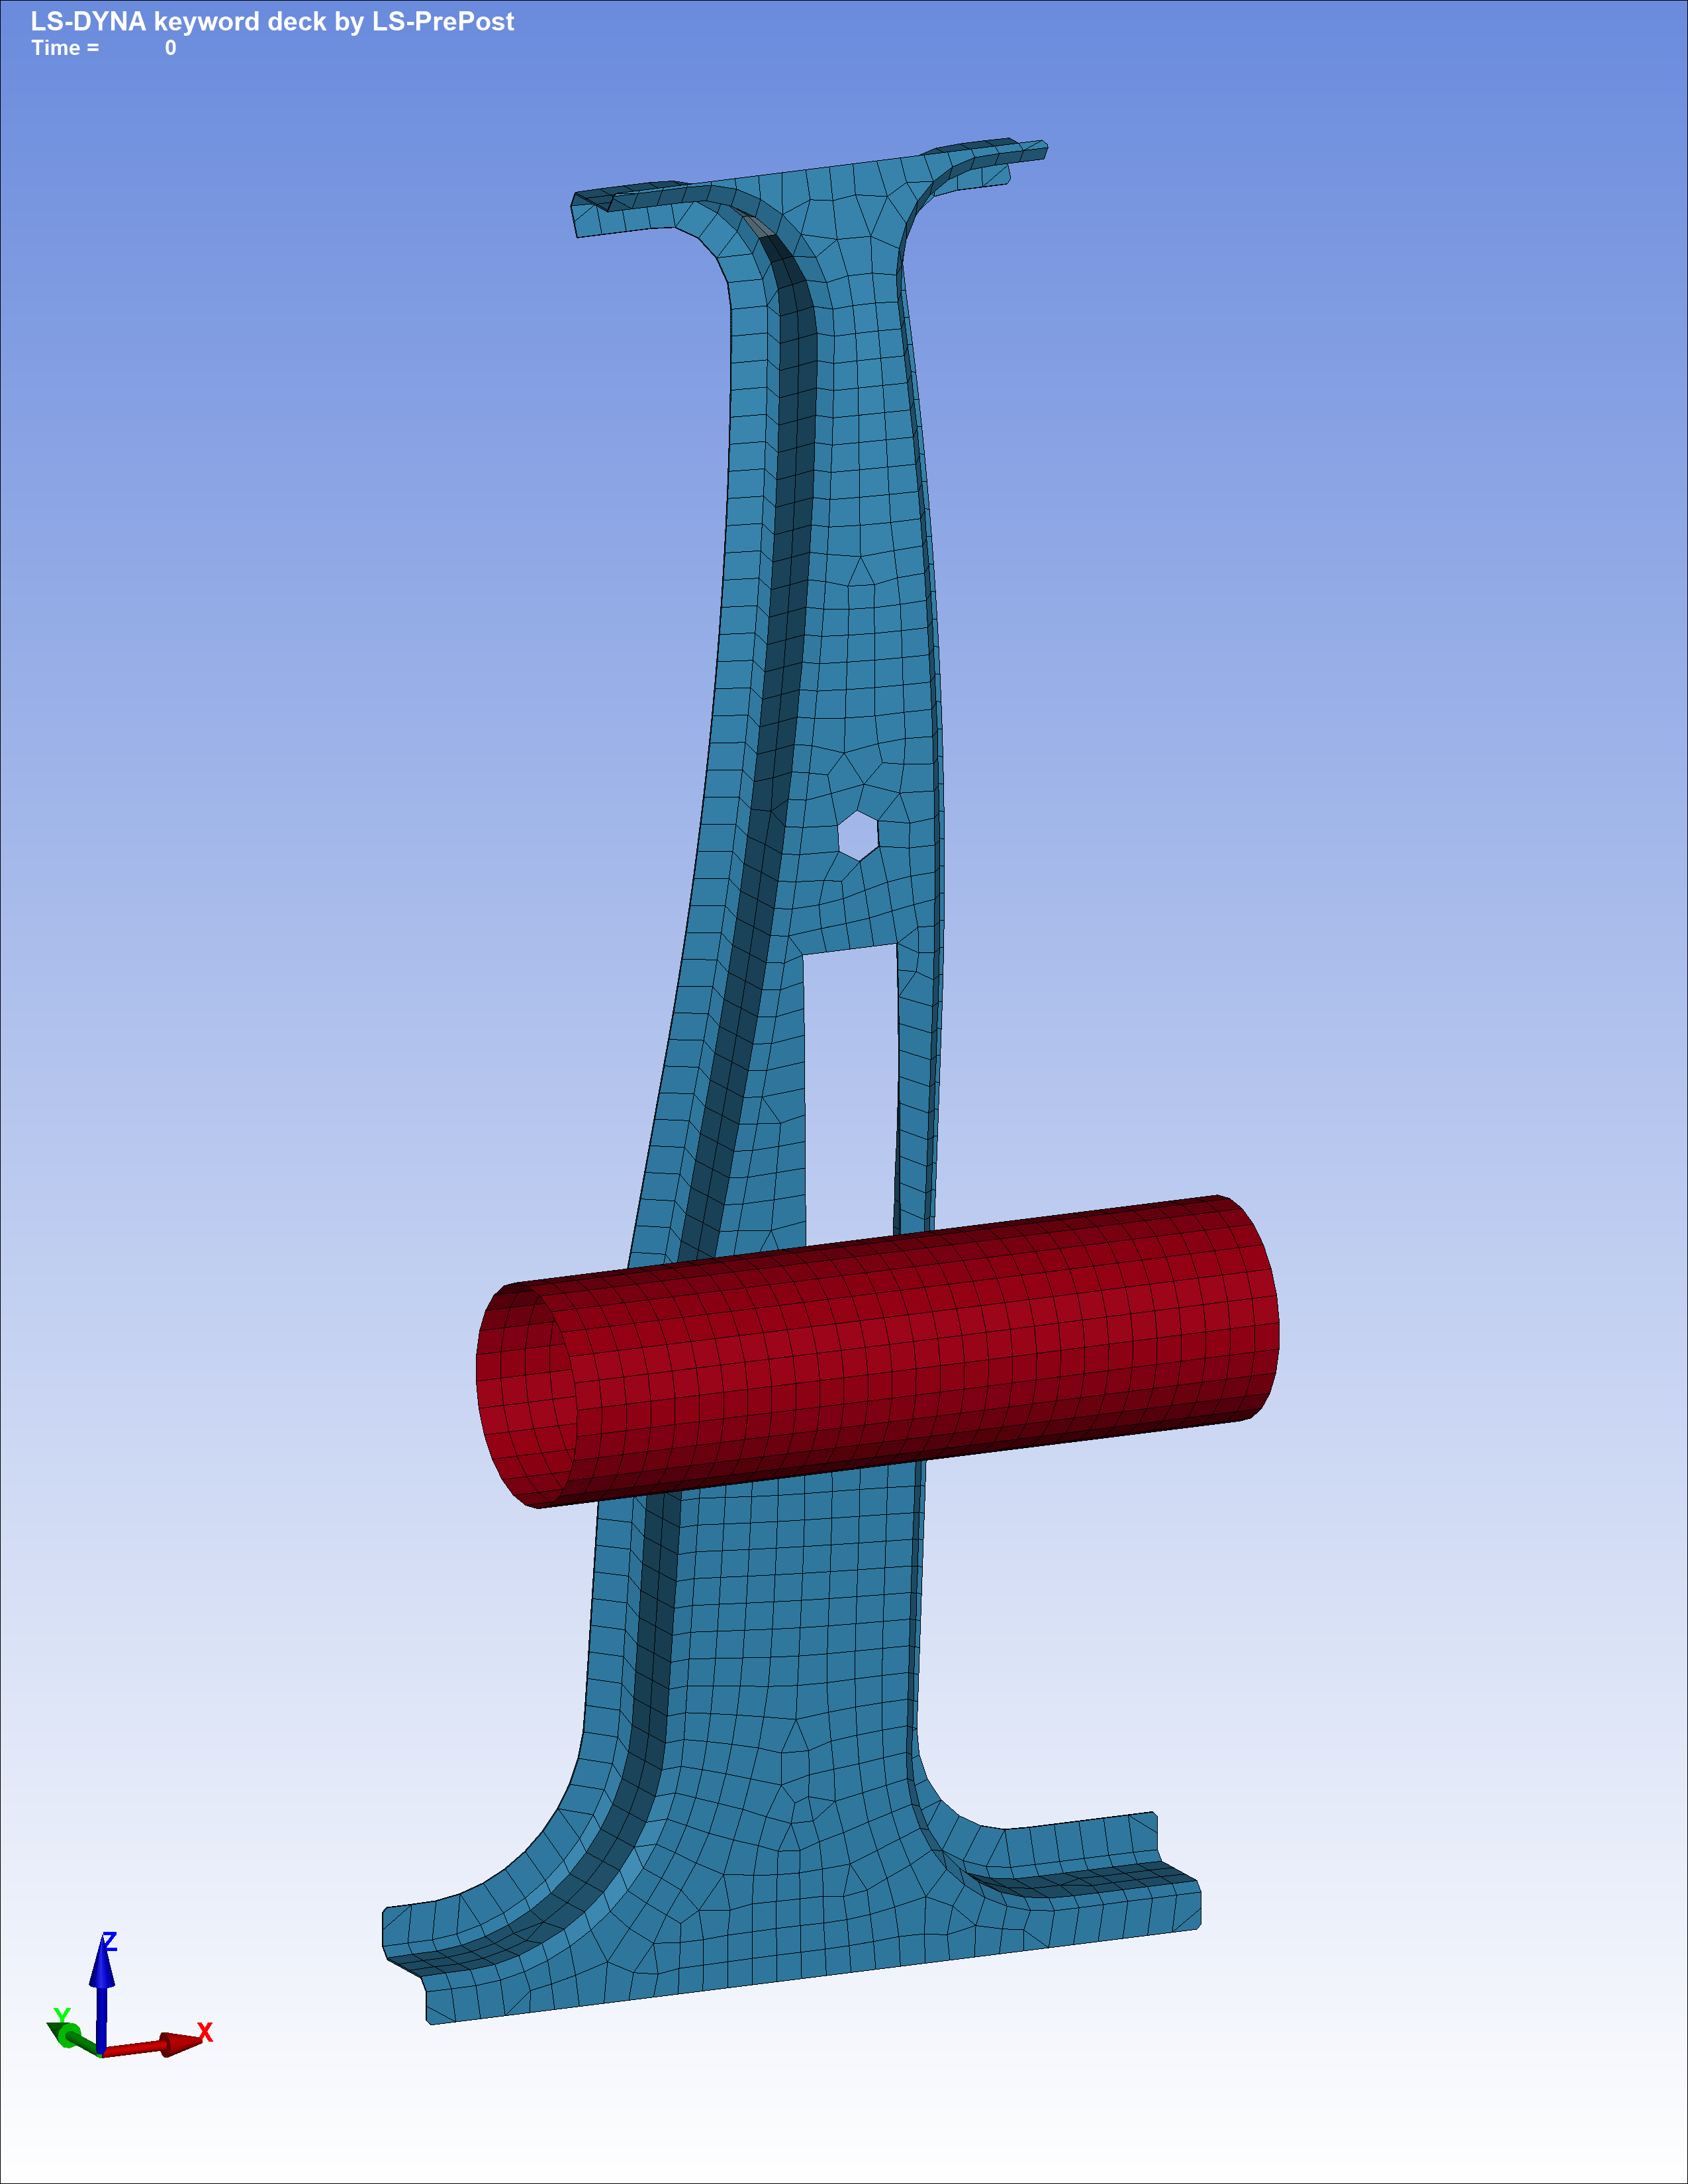
\includegraphics[scale=0.07]{images/modelo-inicial.png} % nombre del archivo
\caption{Modelo inicial}\label{fig:modelo-inicial}
\end{figure}


\begin{figure}[H]
    \centering
    
    % --- fila 1 ---
    \begin{subfigure}{0.45\textwidth}
        \centering
        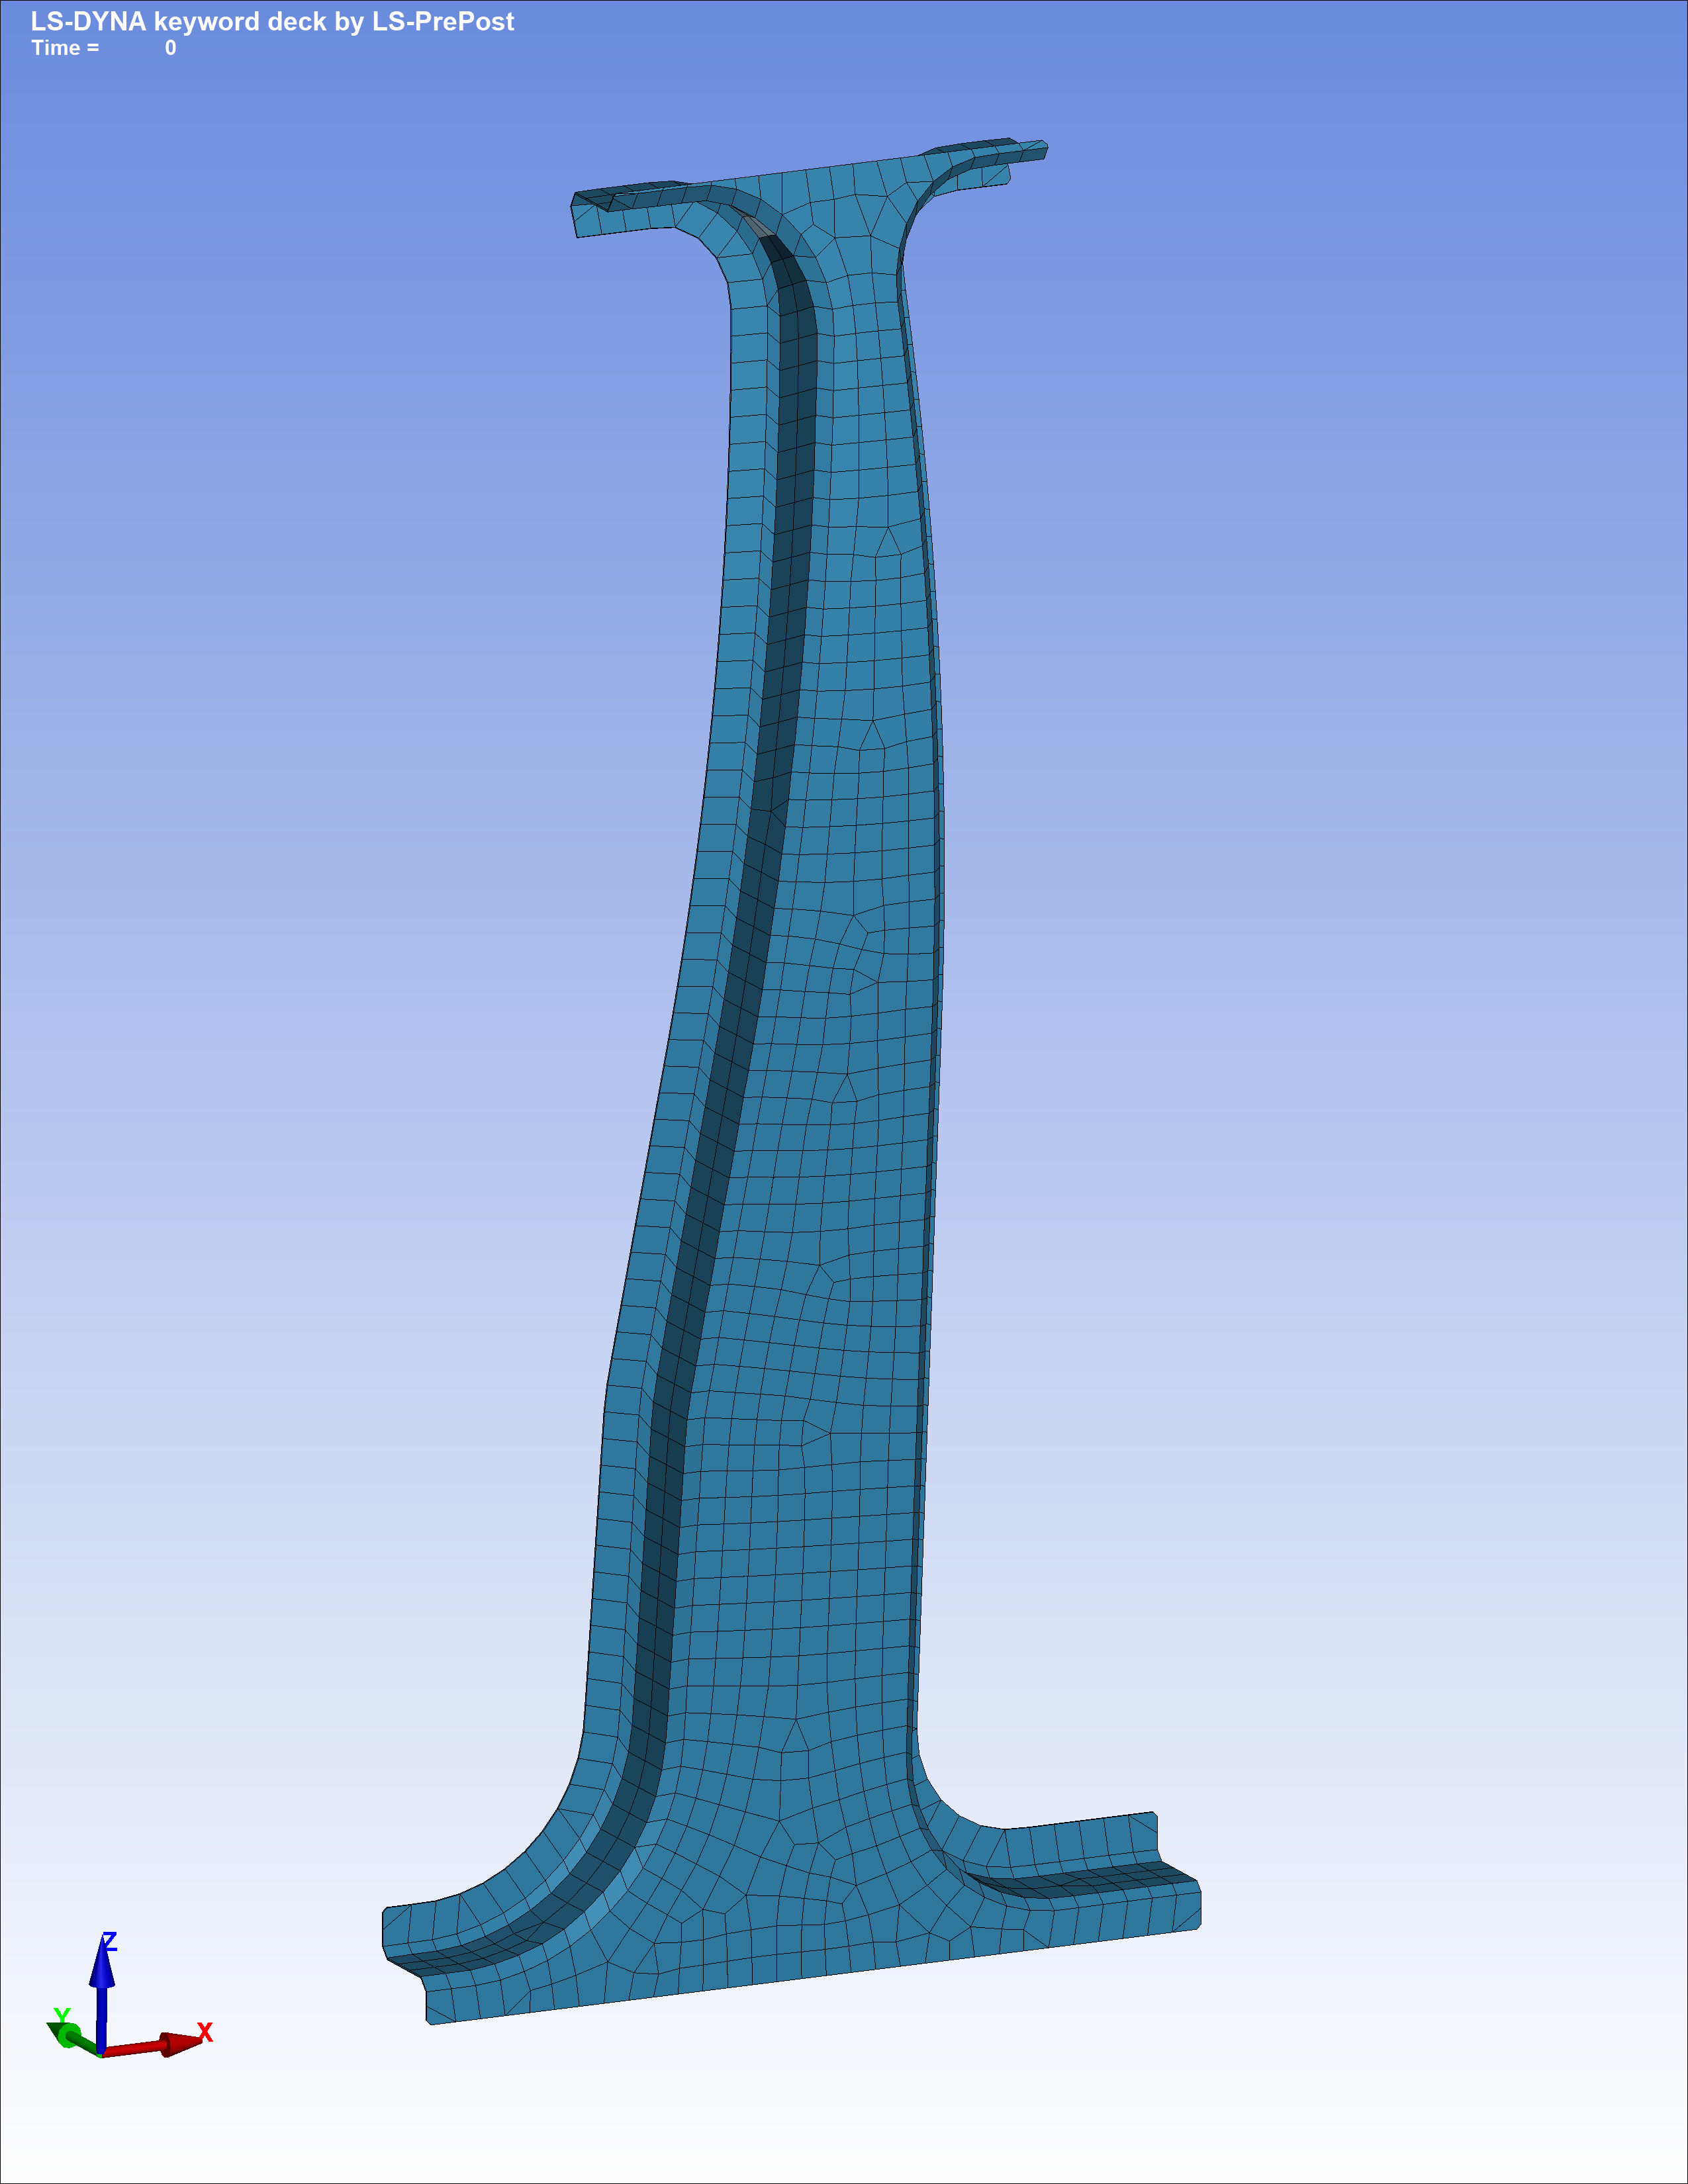
\includegraphics[scale=0.05]{images/b-pillar03.png}
    \end{subfigure}
    \hspace{0.005\textwidth}
    \begin{subfigure}{0.45\textwidth}
        \centering
        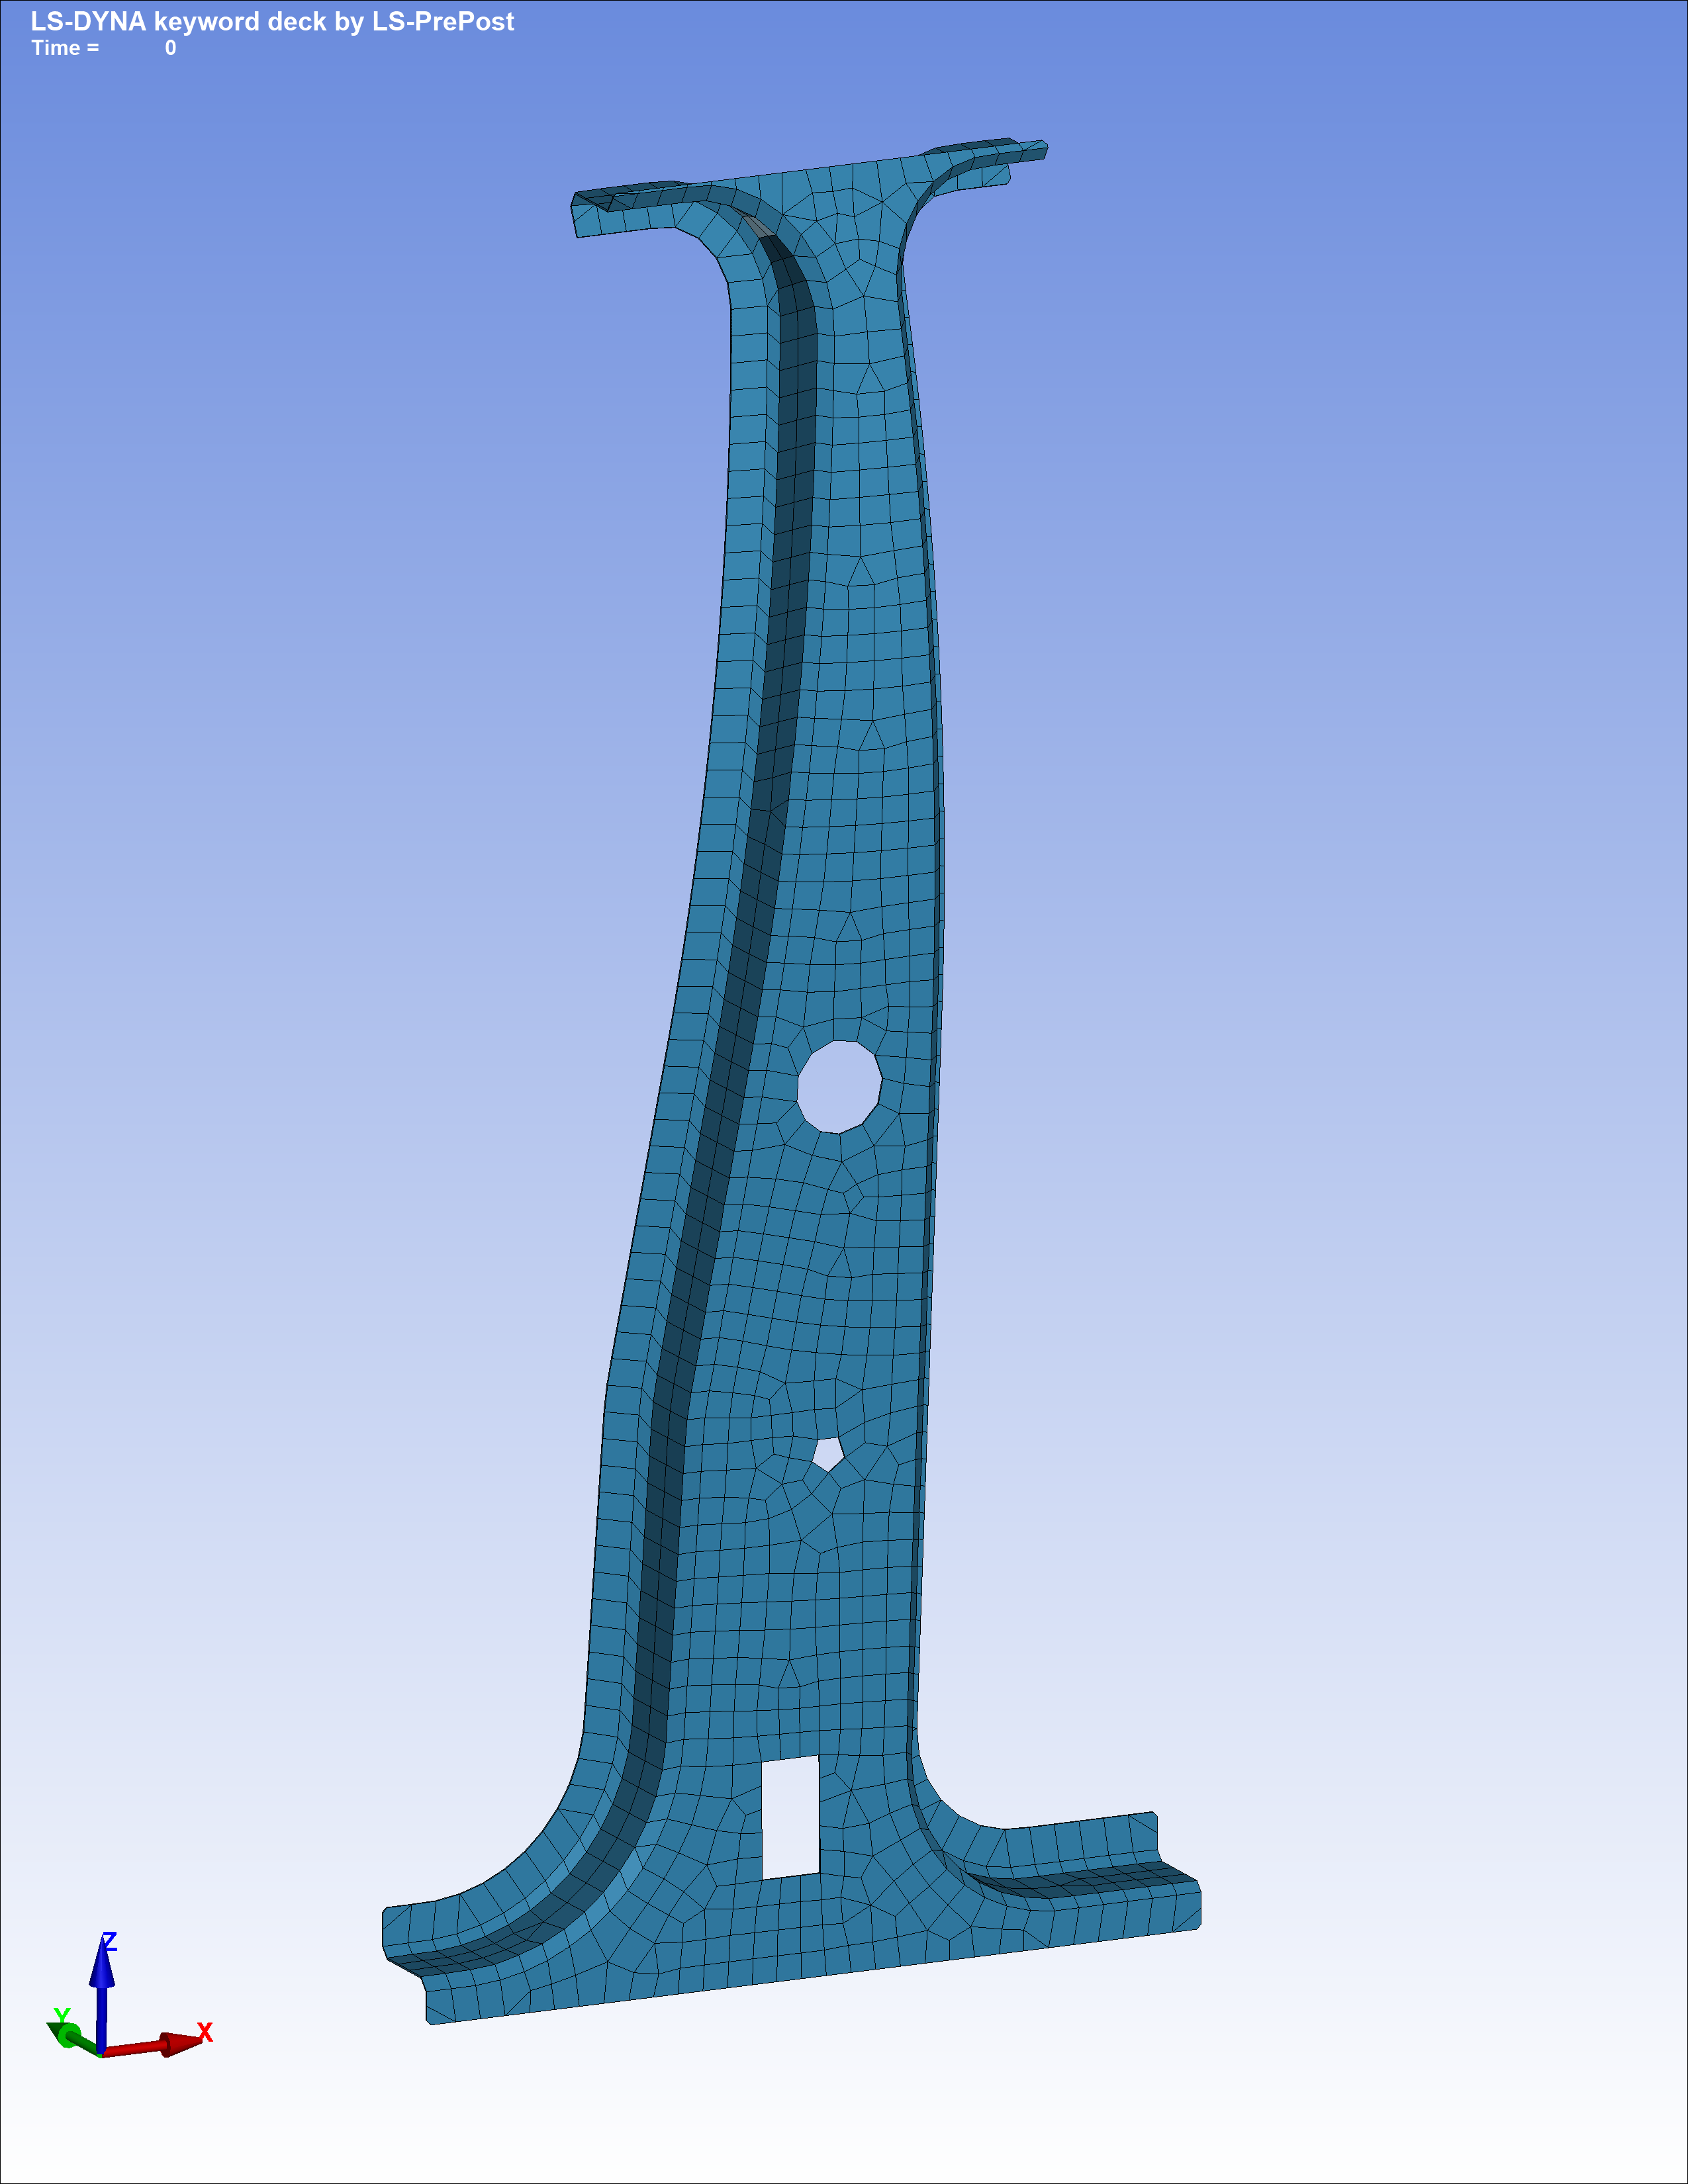
\includegraphics[scale=0.05]{images/b-pillar02.png}
        \end{subfigure}
    
    % --- fila 2 ---
    \vskip\baselineskip
    \begin{subfigure}{0.45\textwidth}
        \centering
        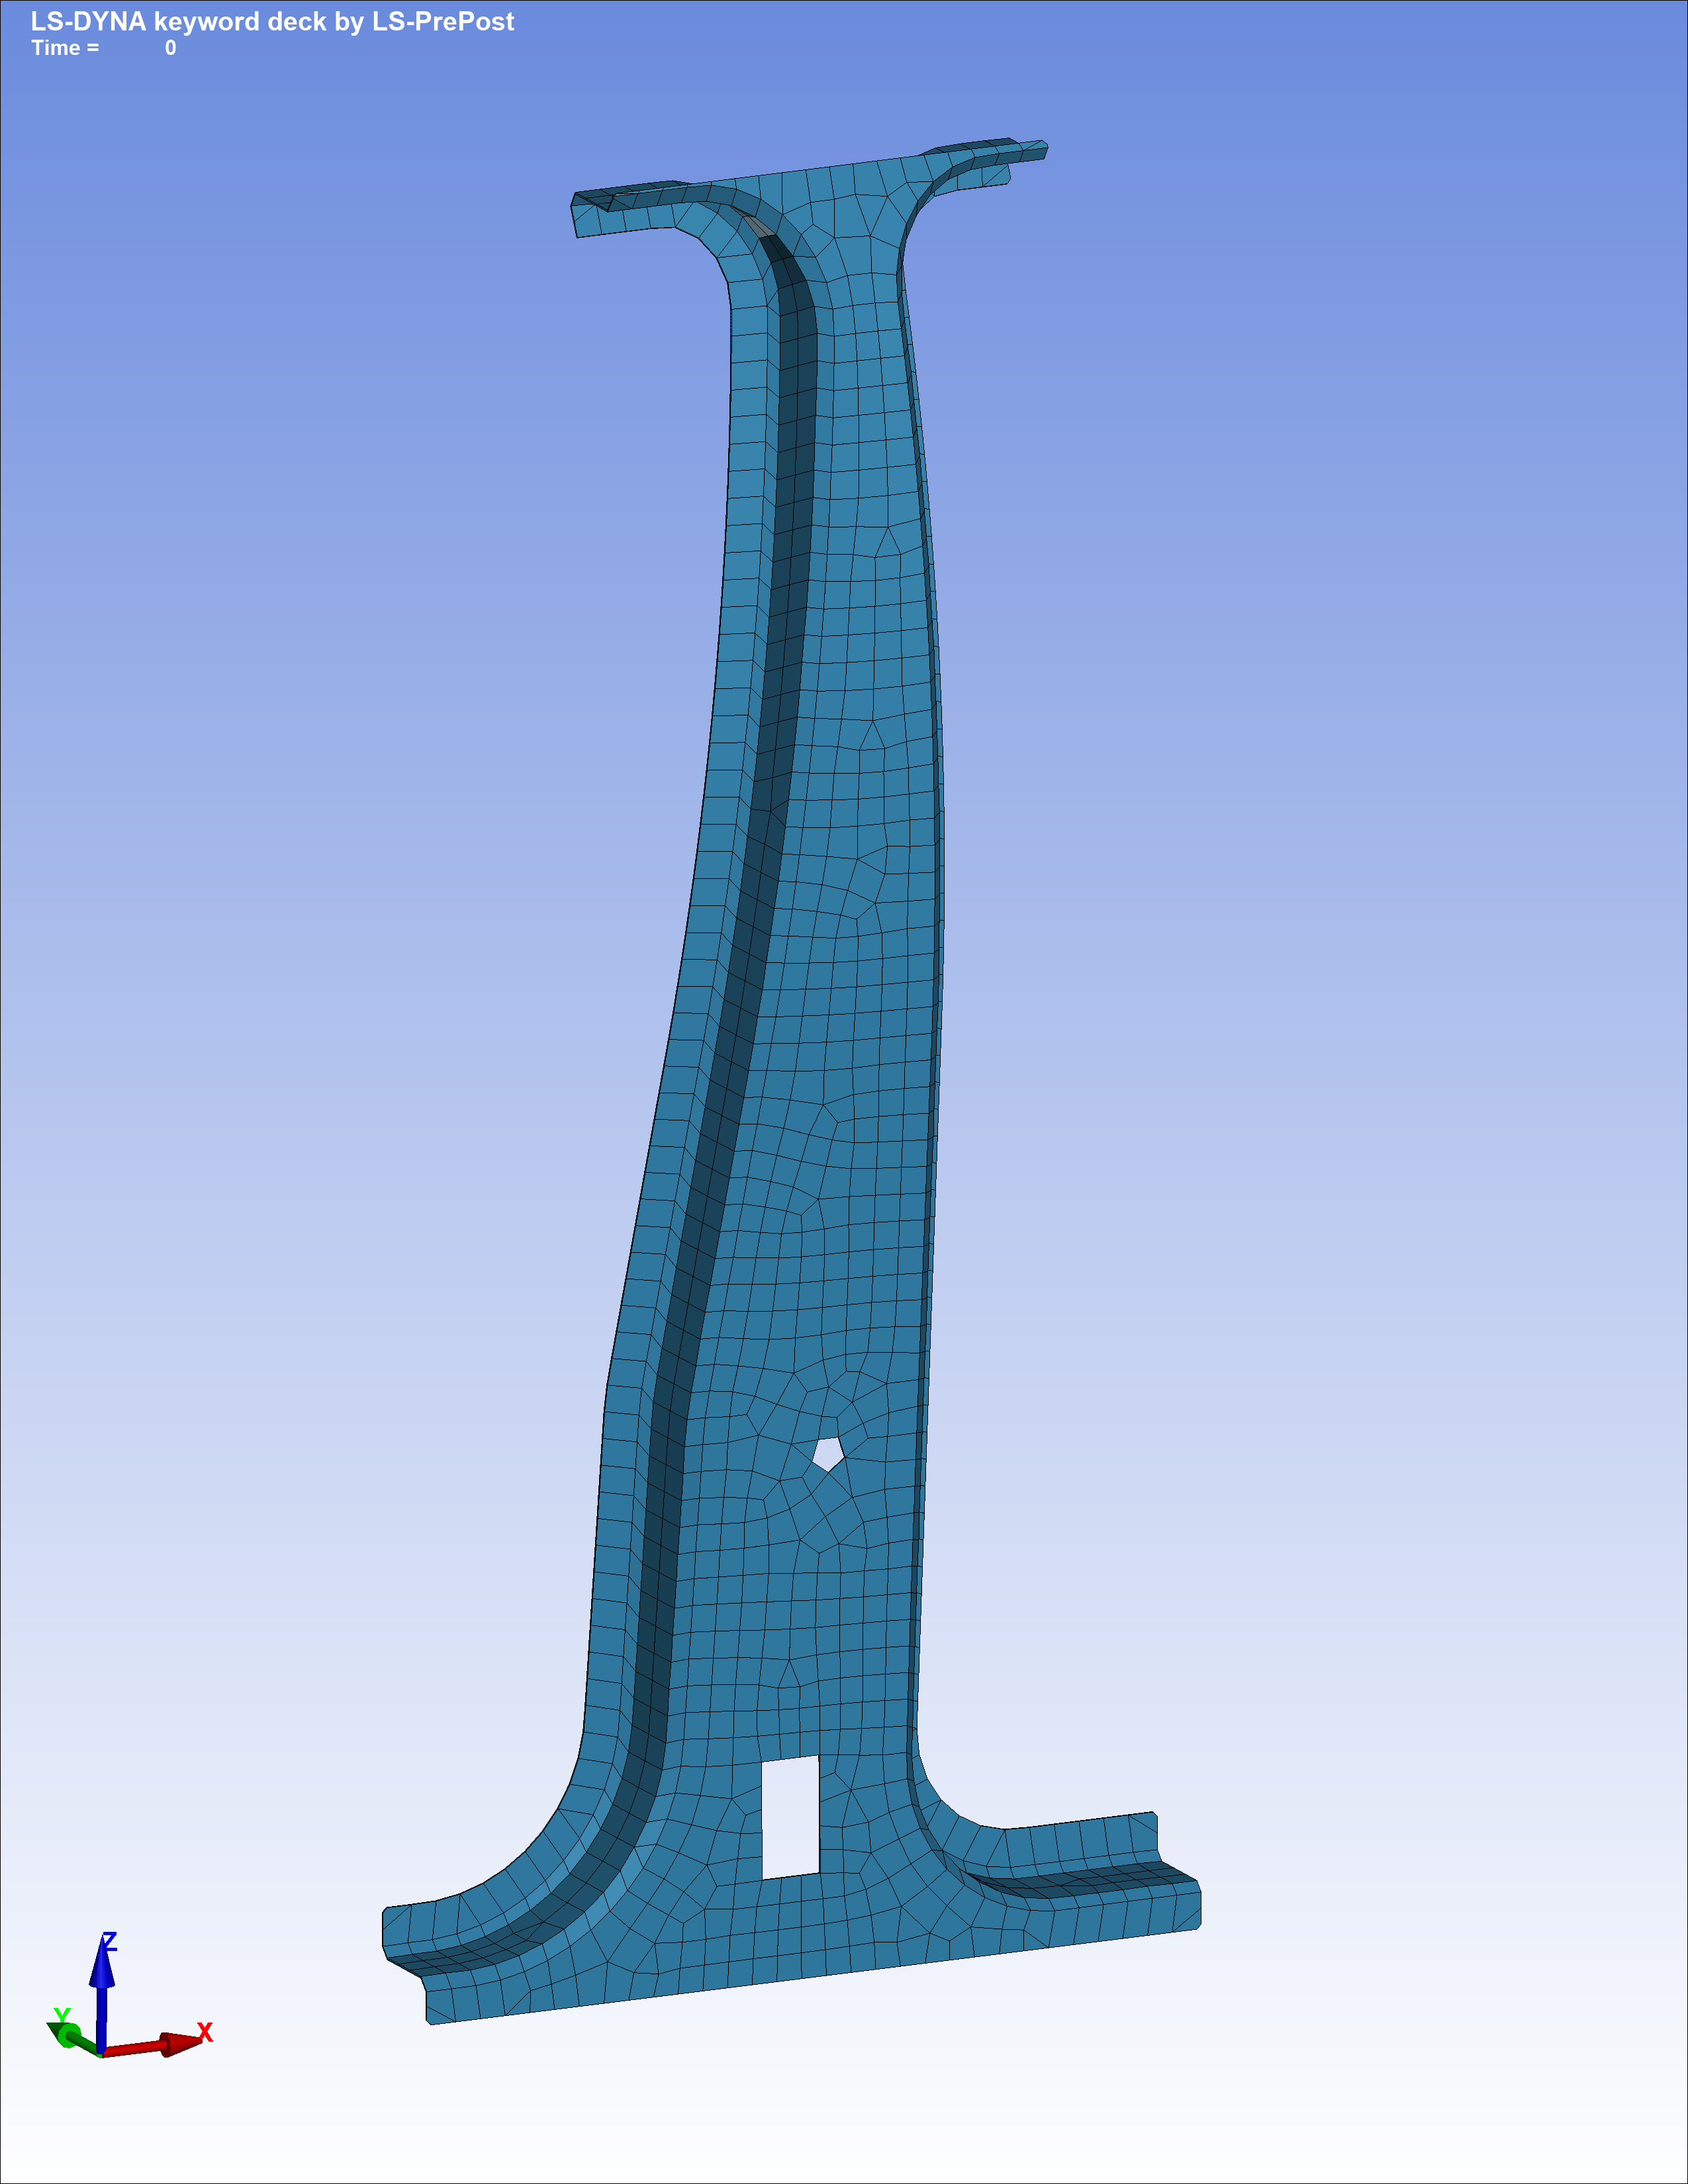
\includegraphics[scale=0.05]{images/b-pillar00.png}
    \end{subfigure}
    \hspace{0.005\textwidth}
    \begin{subfigure}{0.45\textwidth}
        \centering
        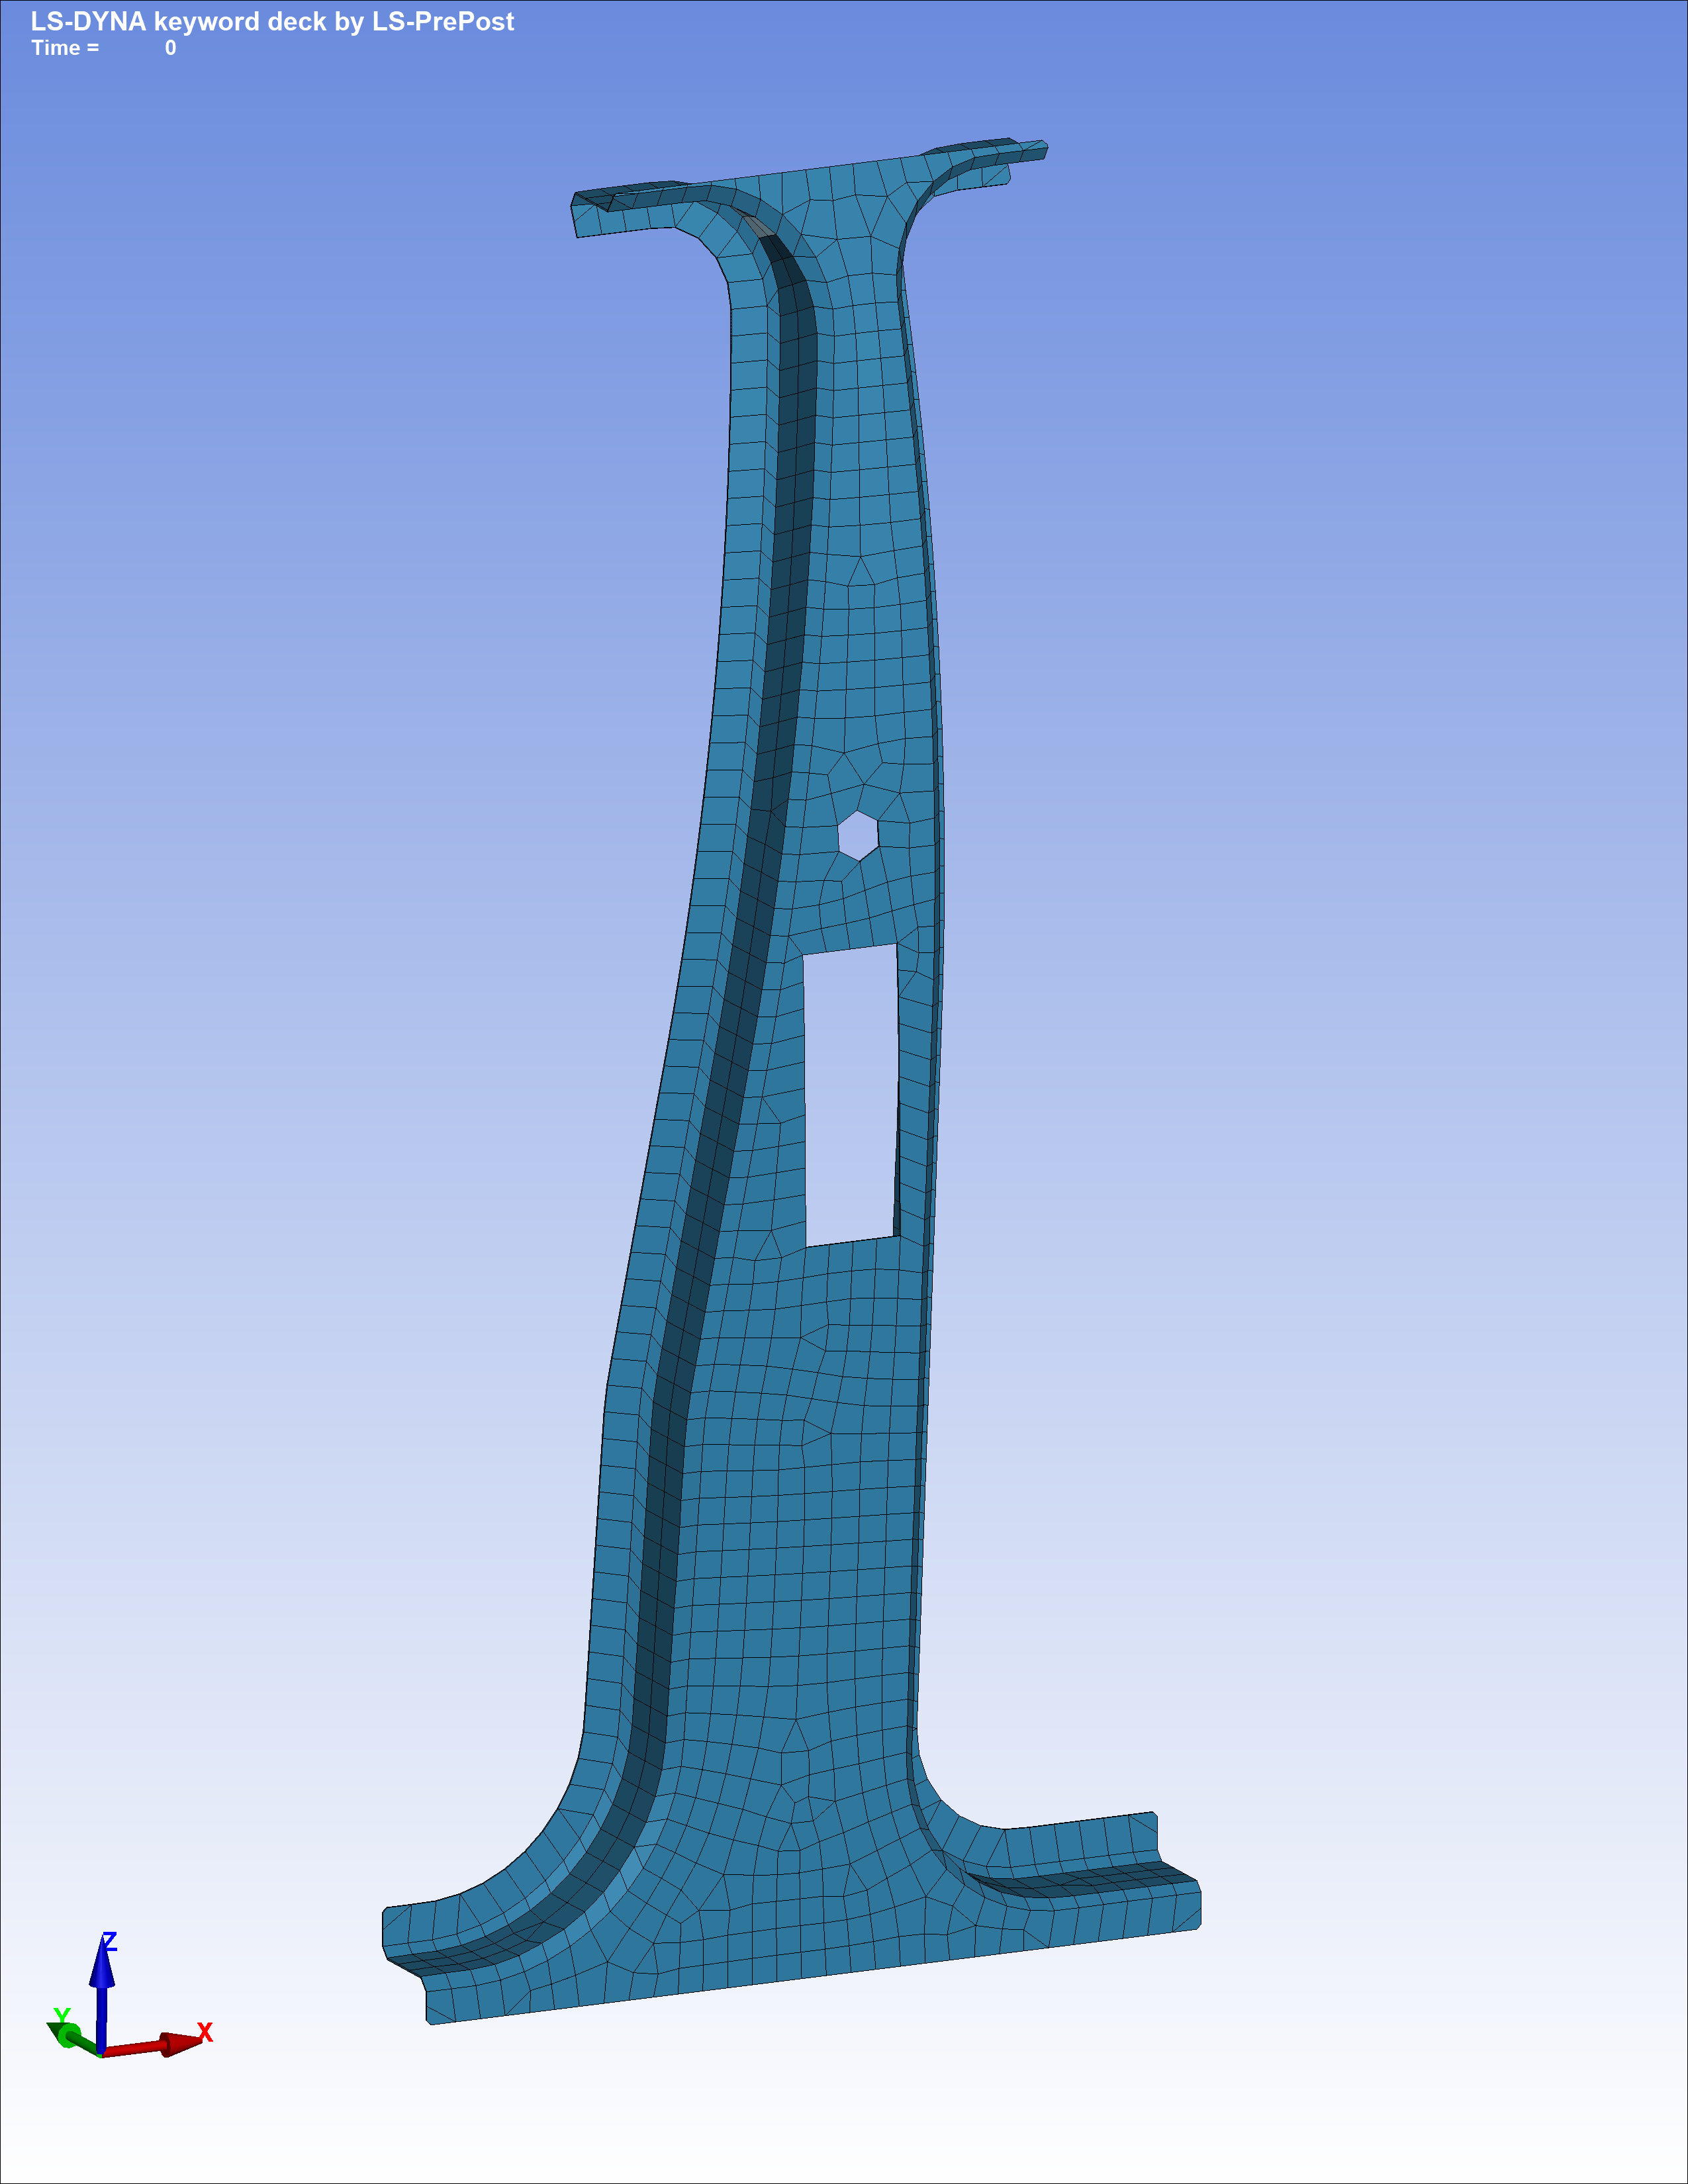
\includegraphics[scale=0.05]{images/b-pillar04.png}
    \end{subfigure}
    
    \caption{Variaciones geométricas del B-Pillar.}\label{fig:variaciones-geometry}
\end{figure}

\subsection{Materiales}
Como materiales para nuestros sólidos elegimos el acero normal para el cilindro impactador y un acero \textit{Ultra High Strenght Steel} (UHSS). La elección de este material se debe a que es 
el estándar usado para elementos críticos de seguridad en la industria automovilística. Además de las propiedades descritas (\cref{tab:materiales})  definimos una cuerva de deformación elástica
para el B-Pillar para simular de la manera más realista posible su deformación a impacto.

\begin{table}[H]
  \centering
  \begin{tabular}{lcc}
    \toprule
    Propiedad & Acero común & UHSS \\
    \midrule
    Densidad (kg/m3)           & 7.85E-6  &  7.85E-6\\
    Módulo elástico (MPa)           & 21000   &  210000\\
    \textit{Poisson's ratio}        & 0.3  & 0.3 \\
    Módulo tangente (MPa)   & 235  & 250 \\
    Tensión de fluencia (MPa) & 1000  & 2100 \\
    \bottomrule
  \end{tabular}
  \caption{Comparación de propiedades entre un acero normal y uno UHSS}\label{tab:materiales}
\end{table}



\subsection{Condiciones iniciales y de contorno}
Como el objetivo del proyecto es estudiar la deformación del B-Pillar y a fin de simplificar los resultados, imponemos que el cilindro se trata de un sólido perfectamente rígido y, por 
tanto, que no sufre ningún tipo de deformación ni elástica ni plástica durante el impacto. Además, para simular que el B-Pillar está anclado al ensamblaje de la matriz del coche, restringimos
el movimiento en todas direcciones en los nodos tanto de la T superior como de la inferior.
Como escenario inicial planteamos uno en el que el B-Pillar se encuentra quieto y anclado y el cilindro irrumpe en su dirección a unos 30 km/h (~10m/s). La elección de la velocidad se debe a que es la 
estándar que se utiliza en estudios físicos de pruebas de impacto.


\subsection{Contacto y fricción}
Dado que tenemos un problema de simulación a impacto, el cálculo preciso y coherente de las potenciales deformaciones que puedan sufrir los cuerpos será una parte crucial de nuestro proyecto.
Para su estudio, LS-DYNA empieza identificando los diferentes cuerpos que componen la simulación (lo que llaman \textit{Parts}). Después, para cada uno de los \textit{timesteps} de la simulación,
utiliza diversos algoritmos a fin de encontrar posibles penetraciones\cite{ls-dyna-contact-support}. En el caso de \textit{penalty-based-contact}, cuando se encuentra una penetración (estudio de las normales), se crea
una fuerza proporcional y opuesta a fin de resistirse y, en último lugar, eliminar dicha deformación. En caso de ser el contacto con un sólido rígido, esa deformación se distribuye de 
manera estatísticamente realista. 
En nuestro proyecto elegimos como modelo de contacto el llamado \textit{Automatic Surface To Surface Contact} debido a que es el estándar y recomendado para este tipo de simulaciones (\cite{ls-dyna-contact-support}).
Este tipo de contacto se diferencia del \textit{One Way Contact} en que aquí se chequea la penetración de los nodos para ambos cuerpos, dando lugar a resultados más precisos. Además,
eliminamos cualquier tipo de posibilidad de "destrucción" o rotura de elementos a fin de evitar oscilaciones numéricas entre simulaciones y facilitar la tarea de predicción al entrenar los
modelos de GNNs. 

\begin{figure}[H] % [h] = here, [t] = top, [b] = bottom
\centering
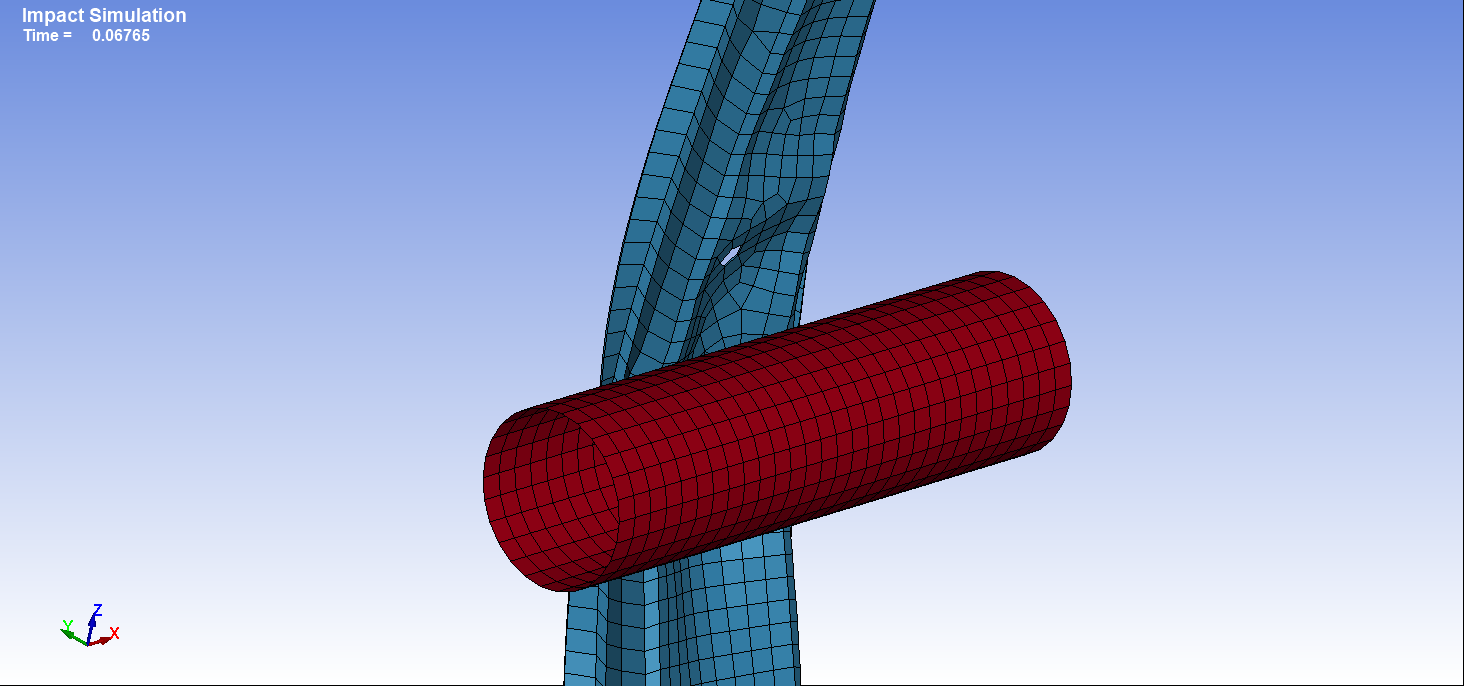
\includegraphics[scale=0.25]{images/impacto.png} % nombre del archivo
\caption{Ejemplo de simulación durante el impacto}\label{fig:simulacion_contacto}
\end{figure}

\subsection{Discretización temporal}
Para la discretización temporal del \textit{solver} LS-DYNA usa variación del método explícito de Diferencias Centrales\cite{ls-dyna-time-integration}.
Este sistema consiste en el uso de los des



% Requiere: \usepackage{amsmath,amssymb}

\section{Integración temporal explícita: esquema de diferencias centrales}

\subsection{Problema dinámico discreto}
La evolución dinámica del sistema FEM se escribe como
\begin{equation}
  \mathbf{M}\,\ddot{\mathbf{u}}(t) + \mathbf{C}\,\dot{\mathbf{u}}(t) + \mathbf{f}_{\mathrm{int}}\!\big(\mathbf{u}(t)\big)
  = \mathbf{f}_{\mathrm{ext}}(t),
  \label{eq:semi-discreto}
\end{equation}
donde $\mathbf{M}$ es la matriz de masas (tomada \emph{lumped}/diagonal en explícito), $\mathbf{C}$ el amortiguamiento efectivo (p.\,ej., Rayleigh o viscosidad artificial) y $\mathbf{f}_{\mathrm{int}}$ agrupa las fuerzas internas (constitutivas) y, cuando aplica, las de contacto.

\subsection{Esquema de diferencias centrales (leap-frog)}
Discretizando el tiempo con paso $\Delta t$, el esquema explícito de diferencias centrales actualiza aceleraciones, velocidades a semipasos y desplazamientos como
\begin{align}
  \mathbf{a}^{\,n} &= \mathbf{M}^{-1}\!\left(\mathbf{f}_{\mathrm{ext}}^{\,n}
  - \mathbf{f}_{\mathrm{int}}\!\left(\mathbf{u}^{\,n}\right)
  - \mathbf{C}\,\mathbf{v}^{\,n-\frac{1}{2}}\right), \label{eq:accel}\\[2mm]
  \mathbf{v}^{\,n+\frac{1}{2}} &= \mathbf{v}^{\,n-\frac{1}{2}} + \Delta t\,\mathbf{a}^{\,n}, \label{eq:vel}\\[2mm]
  \mathbf{u}^{\,n+1} &= \mathbf{u}^{\,n} + \Delta t\,\mathbf{v}^{\,n+\frac{1}{2}}. \label{eq:disp}
\end{align}
La inversión de $\mathbf{M}$ es trivial al ser diagonal, lo que evita resolver sistemas globales en cada paso.

\paragraph{Inicialización.}
Dadas $\mathbf{u}^0$ y $\dot{\mathbf{u}}^0$, se calcula
\begin{align}
  \mathbf{a}^{\,0} &= \mathbf{M}^{-1}\!\left(\mathbf{f}_{\mathrm{ext}}^{\,0}
  - \mathbf{f}_{\mathrm{int}}\!\left(\mathbf{u}^{\,0}\right)
  - \mathbf{C}\,\dot{\mathbf{u}}^{\,0}\right),\\
  \mathbf{v}^{\,\frac{1}{2}} &= \dot{\mathbf{u}}^{\,0} + \tfrac{1}{2}\Delta t\,\mathbf{a}^{\,0}.
\end{align}

\subsection{Tratamiento del contacto}
En explícito, las fuerzas de contacto (normal penalizada y fricción de Coulomb) se evalúan en la configuración de $t^n$, y se incluyen en $\mathbf{f}_{\mathrm{int}}(\mathbf{u}^n)$ de \eqref{eq:accel}. La fricción con transición estática$\to$dinámica puede modelarse mediante una ley de interpolación exponencial dependiente de la velocidad relativa tangencial.

\subsection{Estabilidad y paso crítico}
El esquema \eqref{eq:accel}--\eqref{eq:disp} es condicionalmente estable. Para un sistema lineal no amortiguado,
\begin{equation}
  \Delta t \;\le\; \frac{2}{\omega_{\max}},
\end{equation}
donde $\omega_{\max}$ es la frecuencia natural máxima. En sólidos y cascarones se usa una cota tipo CFL por elemento:
\begin{equation}
  \Delta t_{\mathrm{cr}} \;\approx\; \min_{e}\frac{\ell_e}{c_e},
\end{equation}
con $\ell_e$ una longitud característica del elemento $e$ y $c_e$ la velocidad de onda del material, p.\,ej.\ $c \approx \sqrt{(K+\frac{4}{3}G)/\rho}$ en 3D (o $c\approx\sqrt{E/\rho}$ en 1D). En la práctica, el código evalúa $\Delta t_e$ por elemento y adopta el mínimo global con un factor de seguridad. Para aumentar $\Delta t$ sin modificar la geometría puede emplearse \emph{mass scaling} selectivo, cuantificando su impacto inercial.

\subsection{Ventajas y limitaciones}
\paragraph{Ventajas.}
\begin{itemize}
  \item \textbf{Costo por paso bajo}: no se ensamblan ni se resuelven sistemas globales; $\mathbf{M}^{-1}$ es diagonal.
  \item \textbf{Robustez} frente a no linealidades fuertes: grandes deformaciones, contacto/fricción, plastificación y daño.
  \item \textbf{Paralelizable} y adecuado para mallas grandes de crash.
  \item \textbf{Segundo orden} en el tiempo (para $\Delta t$ constante y sin amortiguamiento) y buen comportamiento conservativo.
\end{itemize}
\paragraph{Limitaciones y cuidados.}
\begin{itemize}
  \item \textbf{Estabilidad condicional}: $\Delta t$ suele ser muy pequeño; fenómenos cuasiestáticos requieren muchos pasos.
  \item \textbf{Precisión} no garantizada por estabilidad: es necesario resolver adecuadamente escalas de onda y contacto.
  \item \textbf{Hourglass} en integración reducida: activar controles adecuados y monitorizar su energía.
  \item \textbf{Amortiguamiento/viscosidad artificial}: útil para choques, pero altera el balance energético; justificar y calibrar.
  \item \textbf{Mass scaling}: altera inercia local; usarlo selectivamente y reportar su efecto (energías y tiempos característicos).
\end{itemize}

% \subsection{Pseudocódigo (operativo)}
% \begin{verbatim}
% Dado u^0, v^0, Δt
% a^0 = M^{-1}(f_ext(u^0) - f_int(u^0) - C v^0)
% v^{1/2} = v^0 + 0.5 Δt a^0
% Para n = 0,1,2,...
%     f_int^n = fuerzas_material(u^n) + fuerzas_contacto(u^n, v^{n-1/2})
%     a^n = M^{-1}(f_ext^n - f_int^n - C v^{n-1/2})
%     v^{n+1/2} = v^{n-1/2} + Δt a^n
%     u^{n+1}   = u^{n} + Δt v^{n+1/2}
%     (opcional) control de Δt, hourglass, energías y penetraciones
% Fin
% \end{verbatim}







\begin{thebibliography}{9}

\bibitem{ls-dyna-manual}
\href{https://lsdyna.ansys.com/wp-content/uploads/2025/02/ls-dyna_950_manual_s.pdf}{LS-DYNA user's manual.Nonlinear Dynamics Analysis of Structures}

\bibitem{abaqus}
\href{https://discover.3ds.com/de/test-and-validate-your-product-faster-abaqus?utm_medium=cpc&utm_source=google&utm_campaign=202501_glo_sea_de_op51508_labl_brand_eca_all&utm_term=abaqus_T100&utm_content=search&gad_source=1&gad_campaignid=22133132152&gbraid=0AAAAADqOeJQo8cPVO3O8HReFA5xqlsbcV&gclid=Cj0KCQjw8eTFBhCXARIsAIkiuOz0AwZ5HHwXXr4HbZGj1htHy6OLYzP8gmSckCMTtP8vHNiF-u39me0aAgNjEALw_wcB}{ABAQUS}

\bibitem{pam-crash}
\href{https://www.esi-group.com/pam-crash}{PAM-CRASH}

\bibitem{ls-dyna-web}
\href{https://www.ansys.com/products/structures/ansys-ls-dyna?&utm_campaign=product&utm_medium=paid-search&utm_source=google&utm_content=digital_structures_copr15ls_contact_contact-us_ls-dyna-structures-brand-search_1a_en_global|110161841694|677373363295|&campaignid=7013g000000cXBnAAM&utm_term=ls%20dyna&plid=110161841694&cid=677373363295&gad_source=1&gad_campaignid=11358860077&gbraid=0AAAAAD8uywbwCN-W7N_ML-4prX1aoVBCW&gclid=Cj0KCQjw8eTFBhCXARIsAIkiuOwIqdHLABcWvzB601bvPjLYZ5dMRd0H0hiRBGsB2mdnjAoNHMxrZb0aApFCEALw_wcB}{LS-DYNA}


\bibitem{ls-dyna-contact-support}
\href{https://www.dynasupport.com/tutorial/ls-dyna-users-guide/contact-modeling-in-ls-dyna}{LS-DYNA contact support}

\bibitem{ls-dyna-time-integration}
\href{https://www.dynasupport.com/tutorial/ls-dyna-users-guide/time-integration}{LS-DYNA time integration}

\bibitem{nastran}
\href{https://www.autodesk.com/products/nastran}{NASTRAN}

\bibitem{knuth}
Donald E. Knuth,
\textit{The TeXbook},
Addison-Wesley, 1984.

\end{thebibliography}

\end{document}
